\subsection{Training data}
As previously mentioned, we mainly focused on the training of our models with unsupervised learning. There is a lot more data explaining the primary structure of the protein, since this is historically very easy to find, compared to finding secondary structure. \\

\noindent
Since we wanted to replicate the work of UniRep, we also chose to use the UniRef50 as training dataset. This dataset is roughly \~27 million proteins. Since this is way too much data, for our hardware to handle in a reasonable time, we decided to randomly sample 100,000 sequences from the same dataset. \\
Since we didn't know that dataset, we chose to randomly sample the data, instead of taking 100k adjacent samples. We did this to avoid any kind of bias the data could have. for example, the first 100k rows of the dataset could potentially only contain one kind of protein.\\

\noindent
UniRep removed proteins containing amino acid symbols (X, B, Z, J), and sequences longer than 2,000 amino acids\cite{unirep}. In our case, due to limited hardware and computer power, we chose to remove all sequences longer than 500 amino acids, and sequences containing the (X, B, Z, J) amino acids as well.\\

\noindent
With the sample reduction, we ended up having roughly 78,000 protein sequences in our training set.\\

\noindent
The primary structure consists of amino acids. Each amino acid is represented as a char \\ $\in \{A, C, D, E, F, G, H, I, K, L, M, N, O, P, Q, R, S, T, U, V, W, Y\}$. meaning that each protein from the dataset is represented as a sequence of chars, with arbitrary length. Since the length of each sequence varies, we've added a padding element (padding element is '-'); padding this element on all sequences, resulting in all sequences has a 500 feature-length. The following figure, shows the frequency of each amino acid in the whole dataset\\

\begin{figure}[!ht]
  \centering
  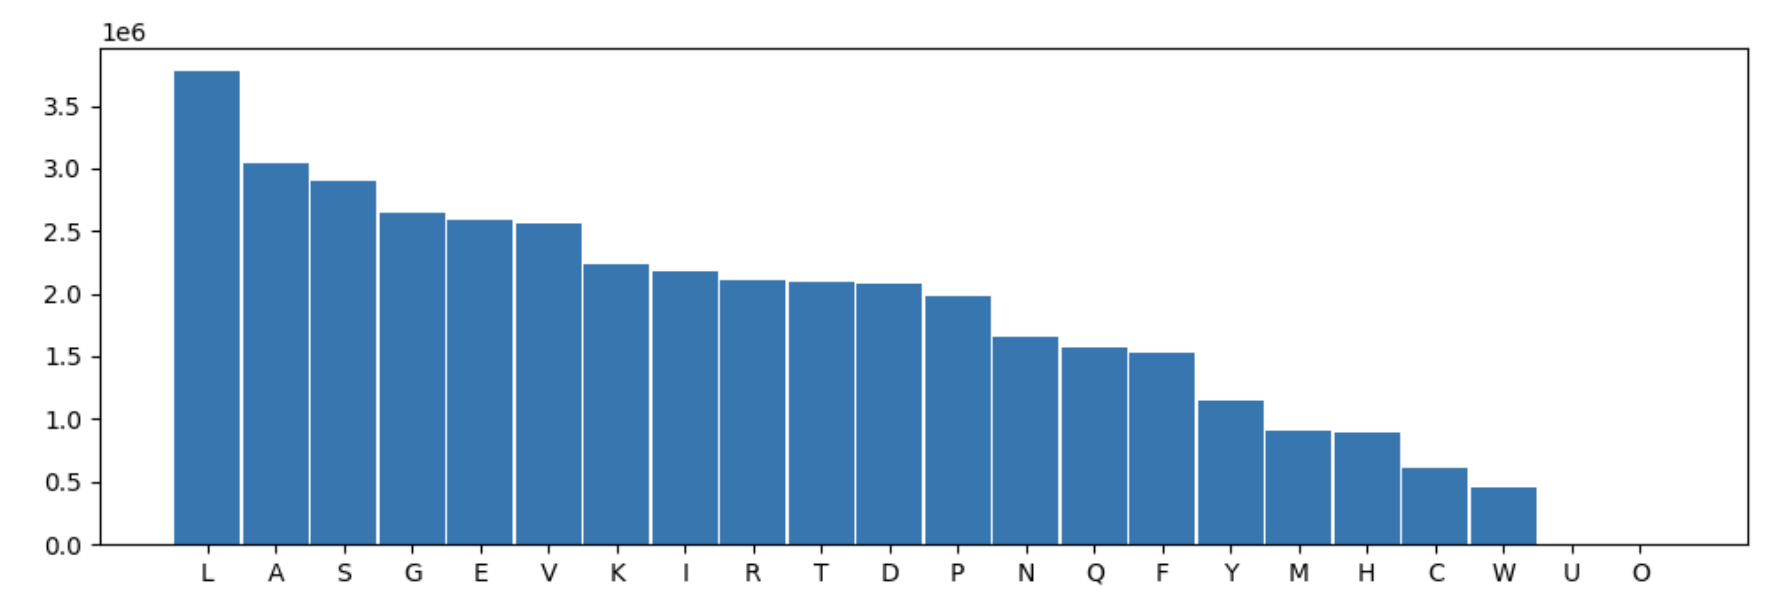
\includegraphics[scale=0.4]{latex/imgs/aminoFreq.png}
  \caption{Histogram of amino acid frequency}\label{Baseline:before}
\end{figure}

\noindent
Our models use embeddings, which is a method of converting a list of one-hot indices, to corresponding word embeddings. In our case, this meant that we had to transform our sequences into one-hot indices. A one-hot encoding is a way to represent the data, through a vector representation only containing \{0,1\}. Say each protein sequence only contain three amino acids (A, C, D), these amino acids will have the following one-hot encodings.

$$
A = \begin{bmatrix}
1 \\
0 \\
0
\end{bmatrix},
C = \begin{bmatrix}
0 \\
1 \\
0
\end{bmatrix},
D= \begin{bmatrix}
0 \\
0 \\
1
\end{bmatrix}
$$

\noindent
If we were looking at four amino acids (A, C, D, E), the one-hot encoding would look like:

$$
A = \begin{bmatrix}
1 \\
0 \\
0 \\
0
\end{bmatrix},
C = \begin{bmatrix}
0 \\
1 \\
0 \\
0
\end{bmatrix},
D= \begin{bmatrix}
0 \\
0 \\
1 \\
0
\end{bmatrix},
E= \begin{bmatrix}
0 \\
0 \\
0 \\
1
\end{bmatrix}
$$

\noindent
We are having working with 22 amino acids and a pad-value each amino acid will be represented $1$x$23$ onehot encoding. The onehot index describes at which index the $1$ is placed. thus if we define the onehot index of any input as $h$, we get:

\begin{align}
h(A) = 0 \\
h(C) = 1 \\
h(D) = 2 \\
h(E) = 3 \\
\end{align}

\noindent
This means our data gets transformed to one-hot indices before we can use it in our models.

\subsection{Labeled data}
Once the model had trained with the training data. We used some labeled data to test the effectiveness of our models. this data also contains protein sequences, but also a label, explaining which structure the protein has. This data made it possible to check if our models can find any separation between the different structures.


\subsection{Stability data}
